% LTeX: language=it
\documentclass[a4paper, 11pt]{article}

%\usepackage{mathrsfs}
\usepackage{amssymb}
\usepackage{amsmath}
\usepackage{array}
\usepackage{epsfig}
\usepackage{float}
\usepackage[margin=2cm]{geometry}
%\usepackage[sectionbib]{chapterbib}
\usepackage{fancyhdr}
\usepackage{lastpage}
\usepackage{graphicx}
\usepackage{caption}
\usepackage{subcaption}
\usepackage{array}
\usepackage{amsfonts}
%\usepackage{color}
\usepackage[usenames,dvipsnames]{color}
\usepackage[hyperindex, linktocpage]{hyperref}
\usepackage[italian]{babel}
\usepackage{wrapfig}

%%%%%%%%%%%%%%%%%%%%%%%%%%%%%%
\newcommand{\class}{Laboratorio di Automatica}
\newcommand{\expT}{Controllo PI di un motore CC}
\newcommand{\repN}{1}
\newcommand{\stud}{Lorenzo Franceschetti, 2000263\\ Leonardo Luigi Pepe, 2009734\\ Federico Saporiti, 2000264}
\newcommand{\dateD}{29 Maggio 2023}

% - Introduzione: modellare motore dc per poi controllarlo con PI
% - Lab 5: modellazione e PI dato
% - Lab 6: calcolo coefficienti PI da specifiche
% - Lab Sperimentale 1: Verifica comportamento

\begin{document}

%\renewcommand{\baselinestretch}{1.5}

\begin{center}
\begin{tabular}{| p{\textwidth} |}
    \hline
    \large
    \vspace{-2pt}
    \stud \hfill
    \Large
    \begin{center}
    {\color{BrickRed}
        \textsl{\class}\\
        \textsl{Relazione n.\repN: \expT}\\
        \large
        \dateD}
    \vspace{-4mm}
    \end{center}\\
    \hline
\end{tabular}
\end{center}

\section{Introduzione}
\subsection{Scopo dell'attività}
L'obiettivo è quello di creare un modello, tramite MatLab e Simulink, di un motore in cc e di progettare un controllore PI rispettando delle specifiche assegnate, in modo da poter controllare la velocità del motore, per poi verificare sperimentalmente in laboratorio che il comportamento reale del motore sia congruo a quello atteso.
\subsection{Organizzazione della relazione}
La relazione si divide in 2 parti: nella prima si crea il modello Simulink del motore in modo da poter eseguire le simulazioni necessarie per verificare il comportamento del controllore prima di applicarlo al motore reale. Questo modello viene poi retroazionato applicando un controllore P e successivamente PI, in modo da evidenziarne il diverso comportamento e valutare la tipologia migliore da usare. Nella seconda parte, invece, partendo da delle specifiche nel dominio del tempo del sistema in catena chiusa, si ricavano i parametri del controllore da usare per il controllo in velocità del motore, con seguente verifica sul modello precedentemente sviluppato. In seguito, si procede alla verifica sperimentale del comportamento del controllore, usando Simulink in tempo reale per controllare il motore elettrico fornito in laboratorio.

\section{Modellazione del motore tramite Simulink}
\subsection{Disegno del modello}
Partendo dalle equazioni che regolano la dinamica elettrica e meccanica del motore, sia dal punto di vista del motore che da quello del carico, si può ricavare un modello del sistema implementabile tramite Simulink. Nel disegnare lo schema, si è tenuto conto delle non idealità del driver di tensione del motore e del convertitore analogico-digitale, come saturazione e quantizzazione. Per la misura della velocità, si è implementato un sistema composto da tre diversi filtri, uno a tempo continuo del primo ordine, uno a tempo continuo del secondo ordine e uno a tempo discreto. Il programma permette di selezionare quale dei tre usare per calcolare la velocità a partire dalla lettura dell'angolo. In questo modo è possibile valutare quale dei tre fornisce il dato più vicino a quello reale, sia in termini di media che di varianza. Per la risoluzione delle equazioni, si è fatto ricorso a un metodo a passo variabile per la soluzione numerica delle equazioni differenziali che regolano il modello, in particolare si è scelto il metodo $ode45$.
\begin{figure}[H]
    \centering
    \begin{subfigure}{0.3\linewidth}
        \centering
        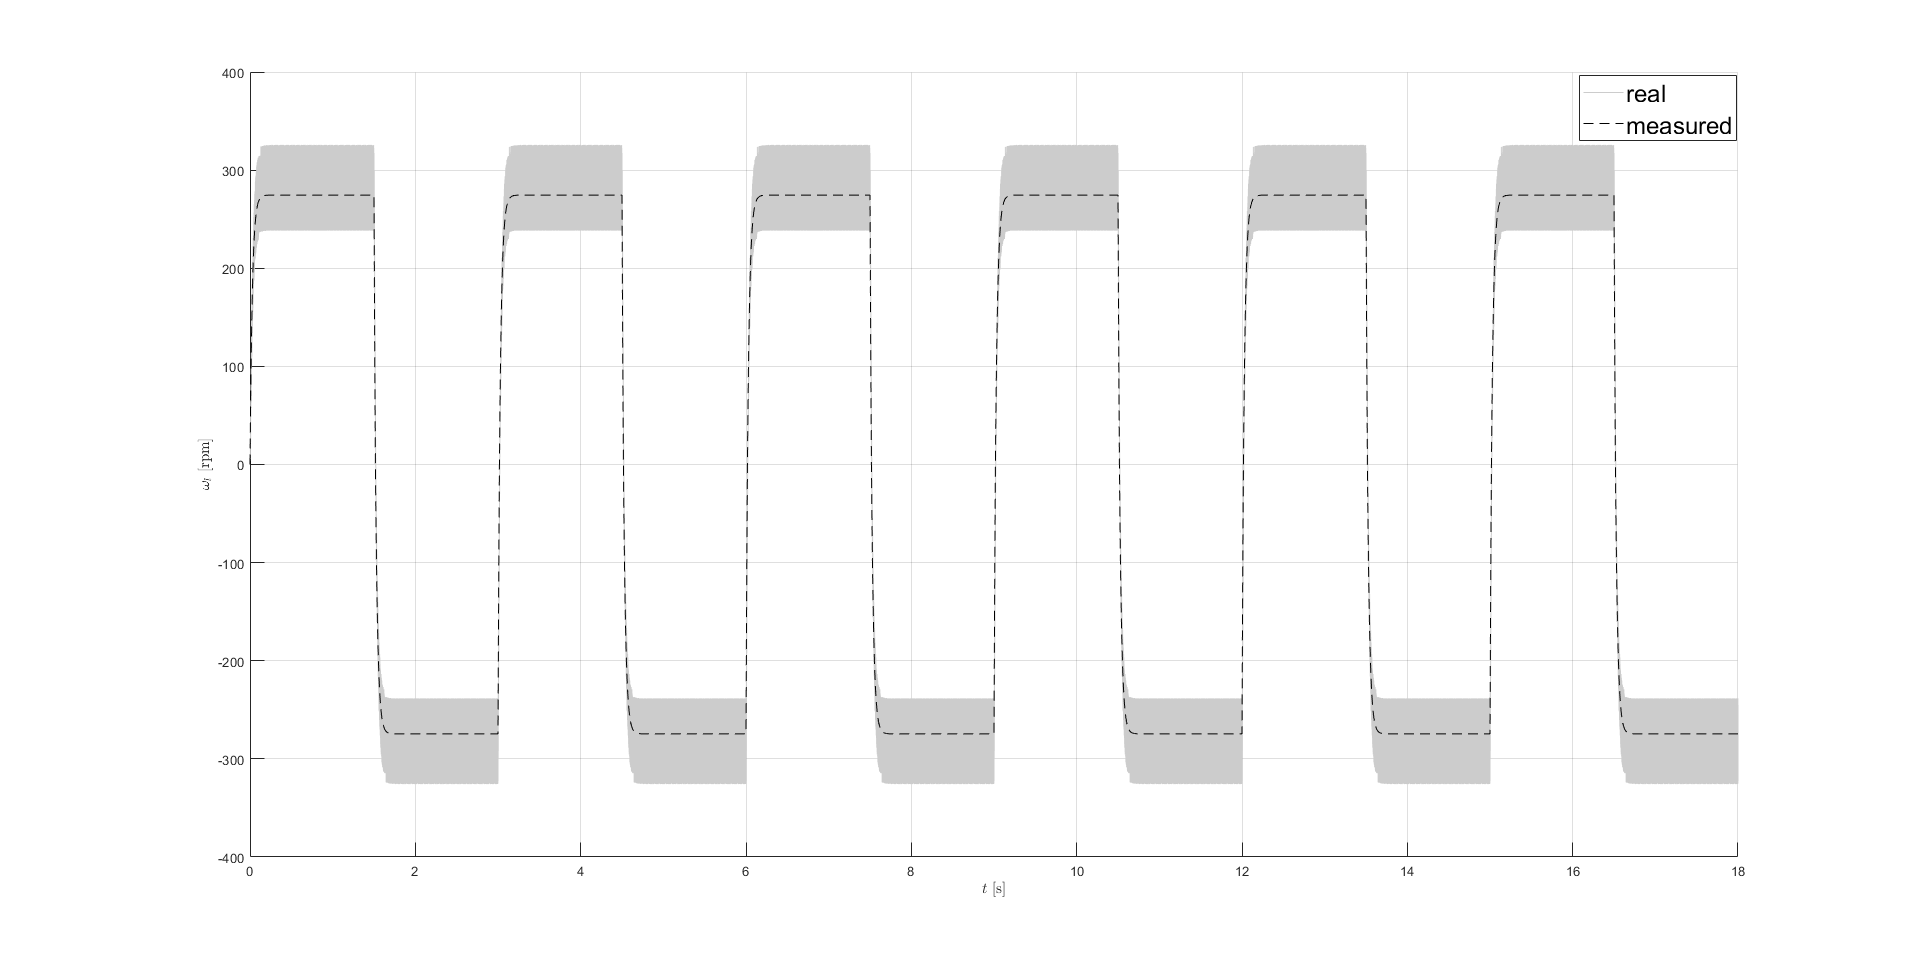
\includegraphics[width=\linewidth]{./Images/speed_filter_1.png}
        \caption{Filtro a tempo continuo del primo ordine}
        \label{Lab5:first}
    \end{subfigure}
    \hfill
    \begin{subfigure}{0.3\linewidth}
        \centering
        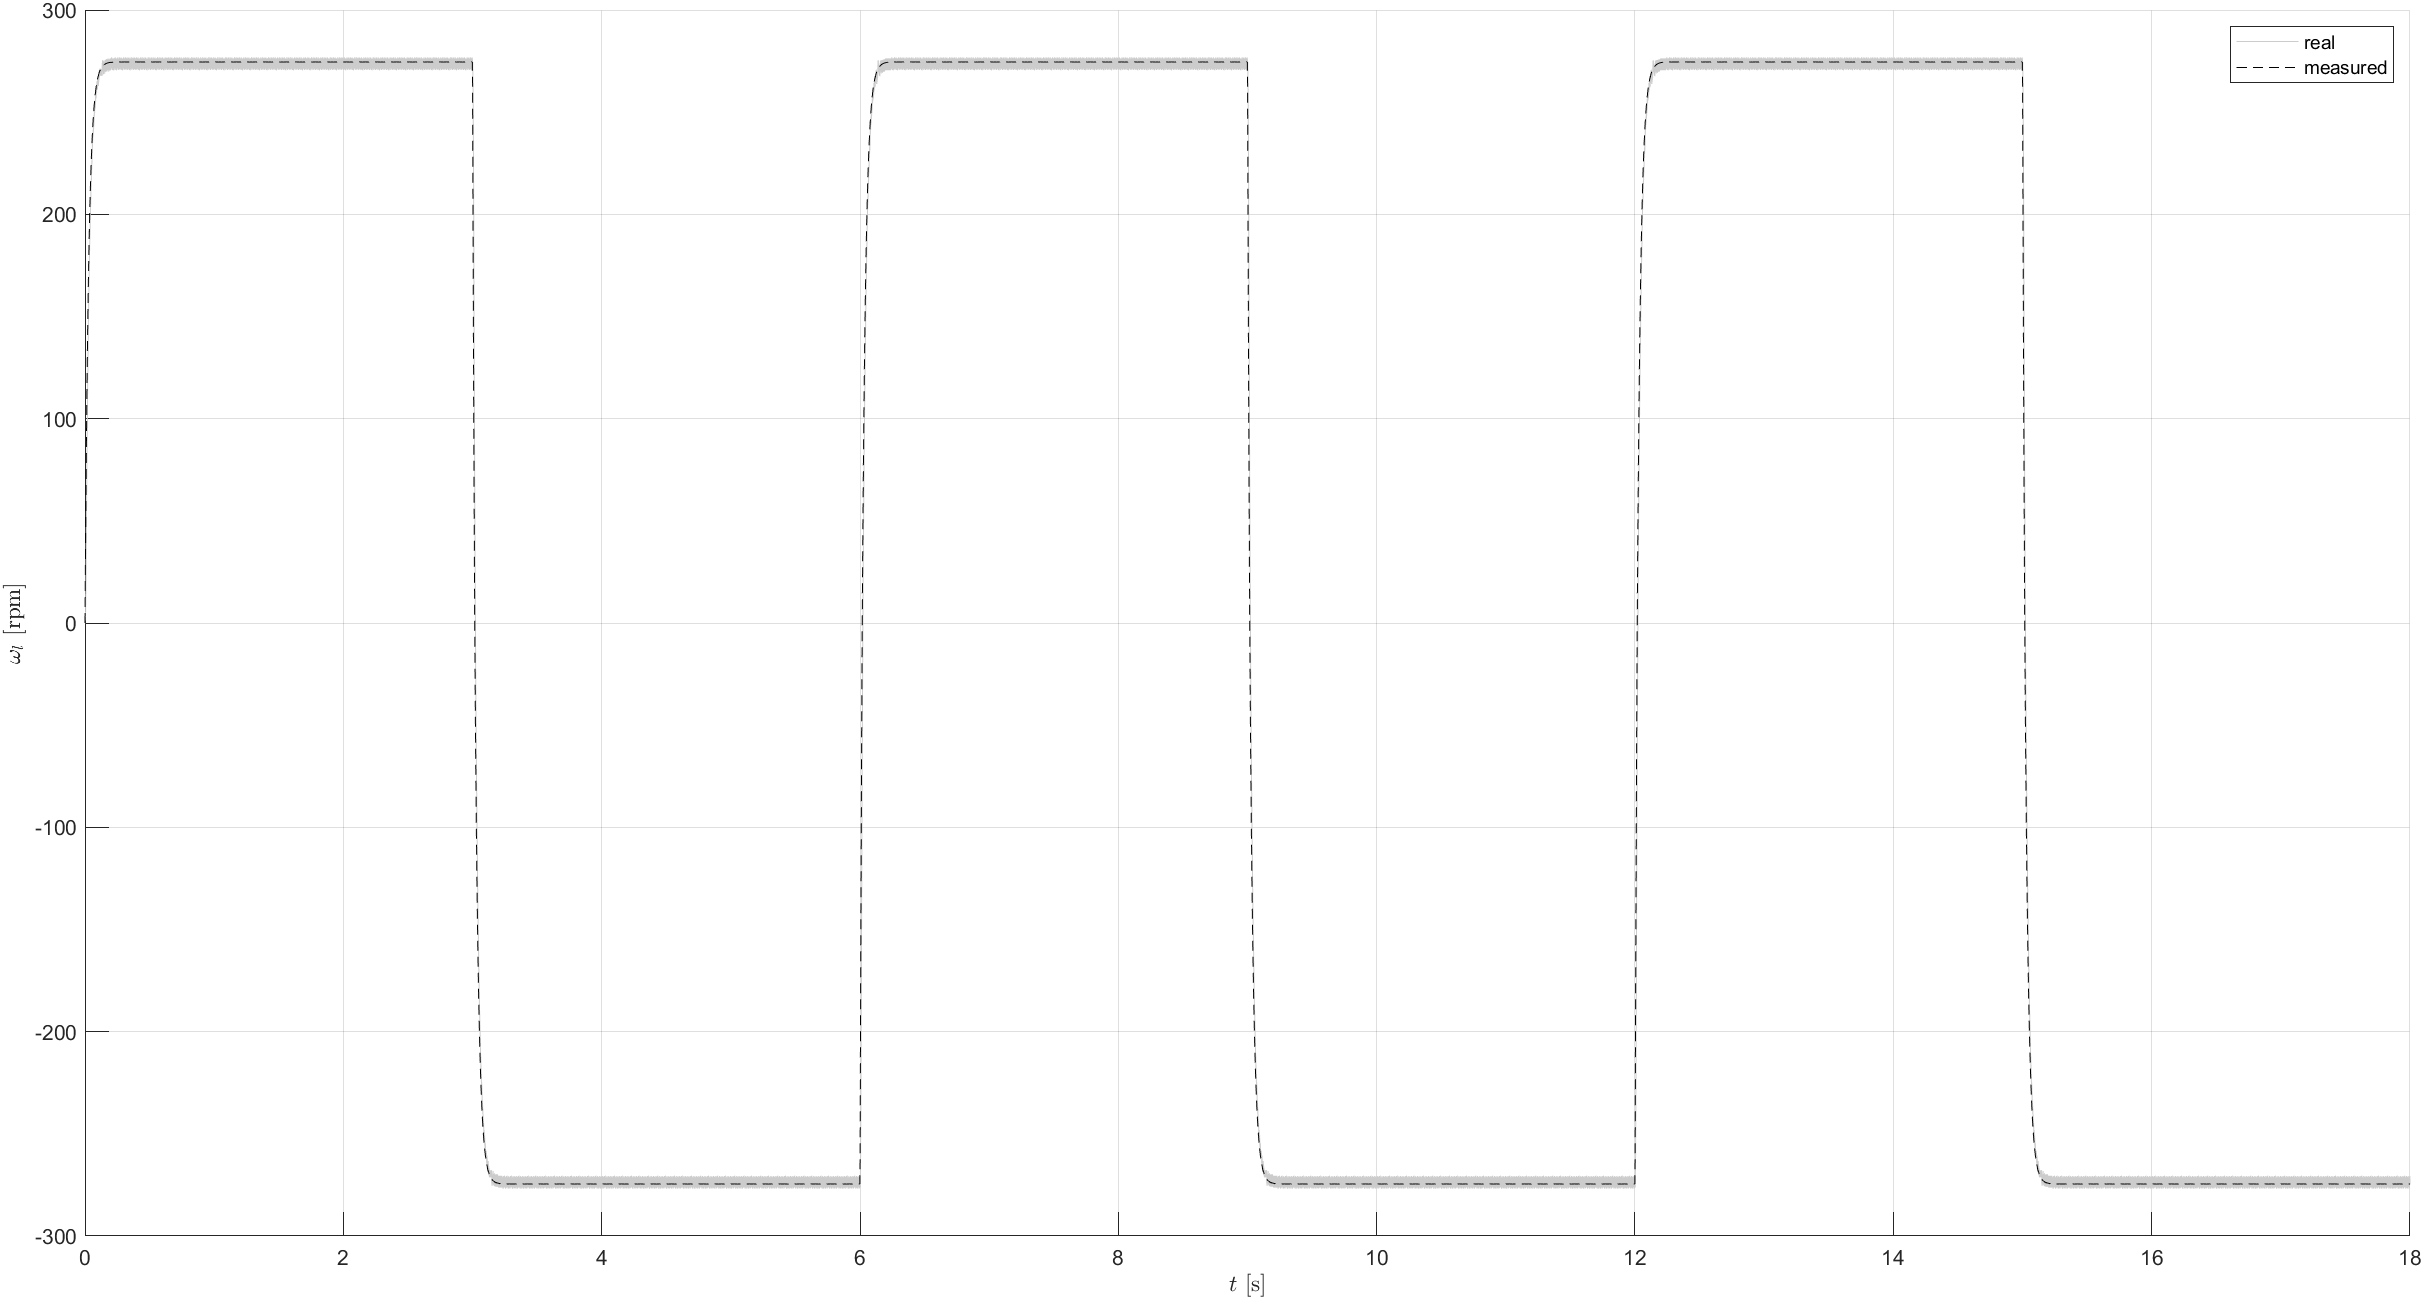
\includegraphics[width=\linewidth]{./Images/speed_filter_2.png}
        \caption{Filtro a tempo continuo del secondo ordine}
        \label{Lab5:second}
    \end{subfigure}
        \hfill
    \begin{subfigure}{0.3\linewidth}
        \centering
        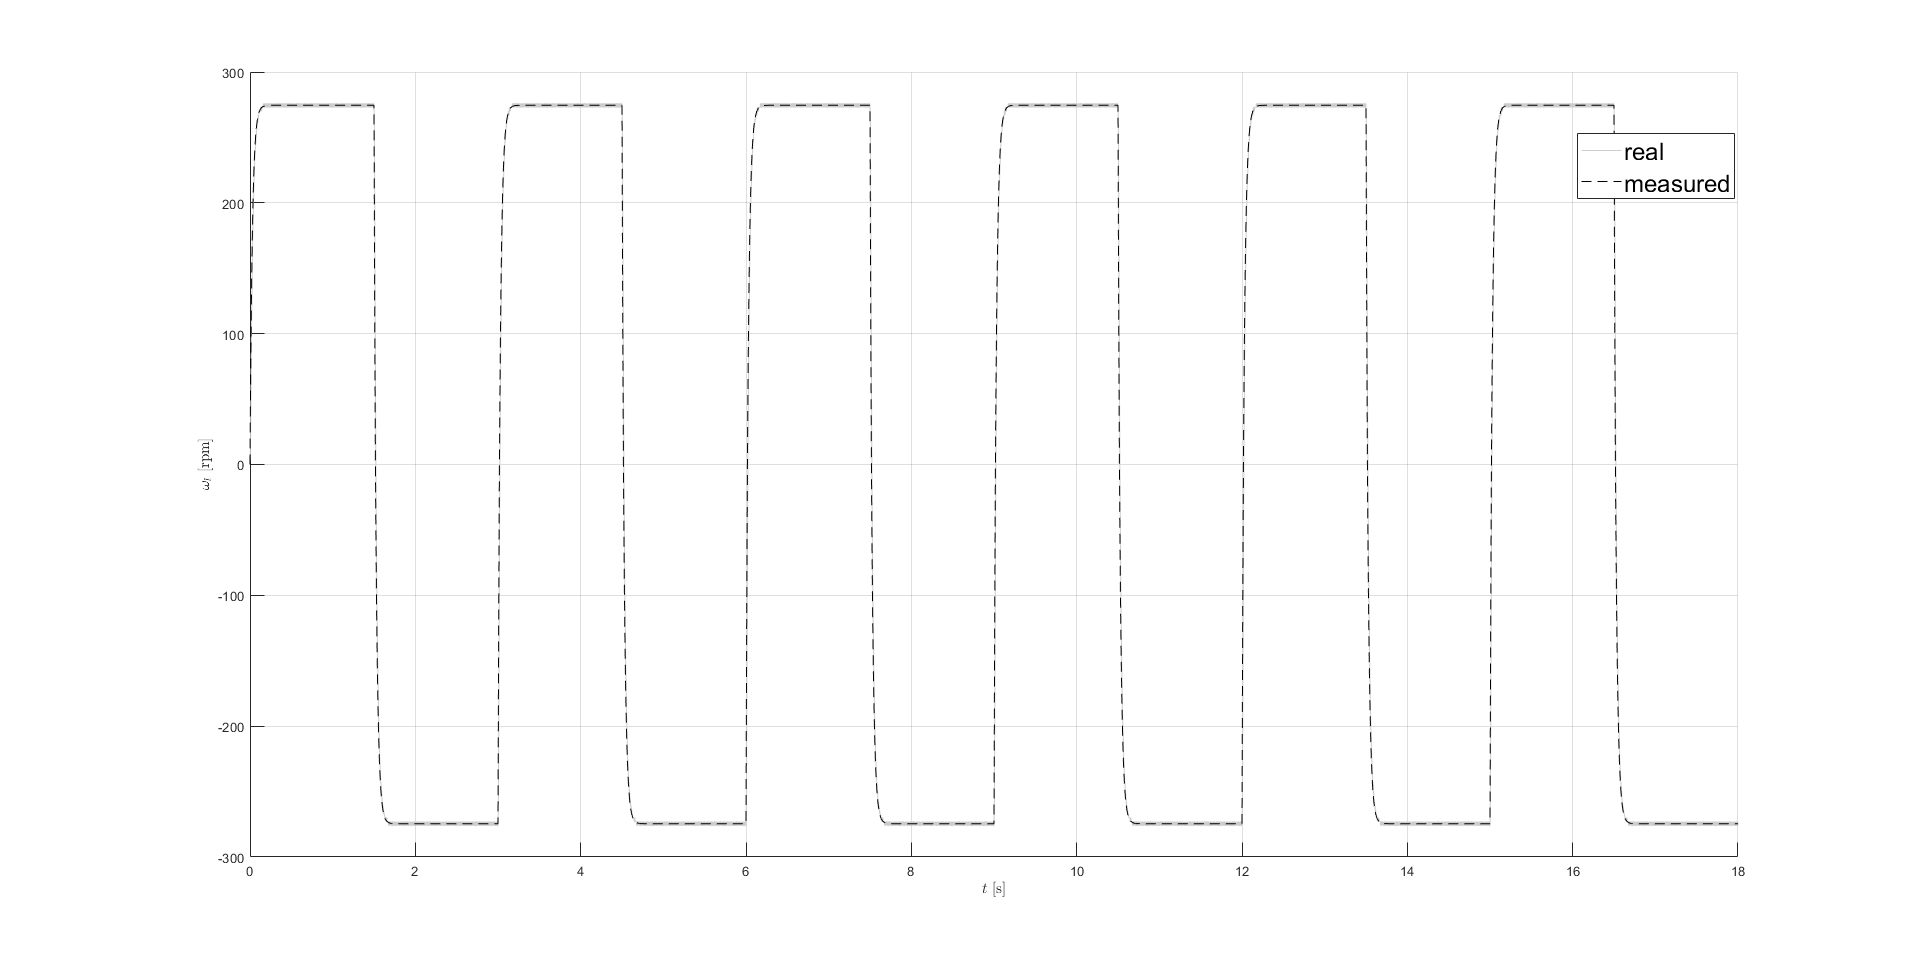
\includegraphics[width=\linewidth]{./Images/speed_filter_3.png}
        \caption{Filtro discreto del decimo ordine}
        \label{Lab5:discrete}
    \end{subfigure}
    \caption{Simulazione velocità}
\end{figure}

\begin{wrapfigure}{r}{0.5\textwidth}
  \begin{center} 
    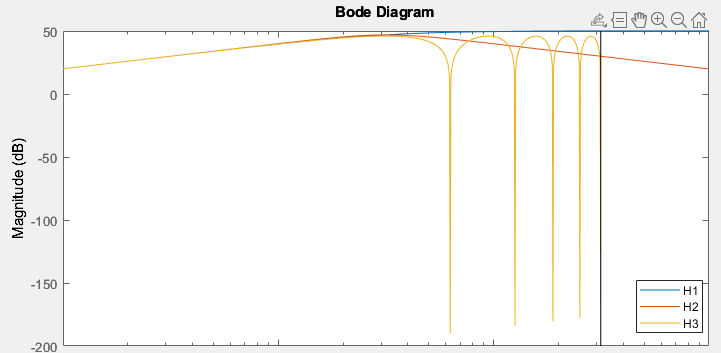
\includegraphics[width=0.45\textwidth]{./Images/speed_filter_responses.png}
  \end{center}
  \caption{Modulo FDT}
  \label{Lab5:mags}
\end{wrapfigure}

Si nota come il filtro del primo ordine dia un risultato molto rumoroso rispetto agli altri due. Infatti, come si ricava dalla figura \ref{Lab5:mags}, il filtro del primo ordine ha modulo quasi costante ad alte pulsazioni, pari a $50 dB$, mentre gli altri due hanno modulo decrescente e quindi riescono a attenuare in maniera più efficiente i disturbi alle alte frequenze, dando un risultato meno rumoroso.

\subsection{Controllo in retroazione di velocità}
Per fare in modo che il motore segua in maniera corretta un segnale di riferimento di velocità, è possibile sfruttare la retroazione con un controllore adeguato, che permetta al sistema di inseguire un segnale costante con errore nullo a regime. Inizialmente, si usa un controllore di tipo P, con costante $K_{P} = 1$, prendendo come segnale di errore la differenza tra il segnale di riferimento, scelto come un'onda quadra di valore $250 rpm$ e periodo $3s$, e la stima della velocità, data da un filtro del secondo ordine. 

Come si può vedere dalla figura \ref{Lab5:P}, il controllore non è in grado di inseguire il riferimento con errore a regime nullo, ma ha un errore costante, che non viene eliminato. Questo è dovuto al fatto che la funzione di trasferimento del sistema originale non presenta poli nell'origine, quindi, se viene messa in retroazione, il sistema risultante è di tipo 0. Il controllore di tipo P, avendo forma $C(s) = K_{P}$, non introduce poli nell'origine, quindi il sistema retroazionato rimane di tipo 0 e presenta un errore costante non nullo se l'ingresso è un segnale a gradino costante. Un modo per eliminare questo errore è passare a un controllore PI, nella forma $C(s) = K_{P} + K_{I} / s$, che introduce un polo nell'origine e aumenta di 1 il tipo del sistema. In questo modo, ottengo un sistema di tipo 1 che presenta, in presenza di un ingresso a gradino, un errore a regime nullo. La conseguenza dell'uso di un PI è la presenza di sovraelongazione iniziale, a causa dell'azione integrale. Il grafico \ref{Lab5:PI} è ottenuto con $K_{P} = 0.01$ e $K_{I} = 1$. Si nota che l'errore a regime è nullo, ma dove il gradino cambia valore si presenta un fenomeno di sovraelongazione.
\begin{figure}[H]
    \centering
    \begin{subfigure}{0.45\linewidth}
        \centering
        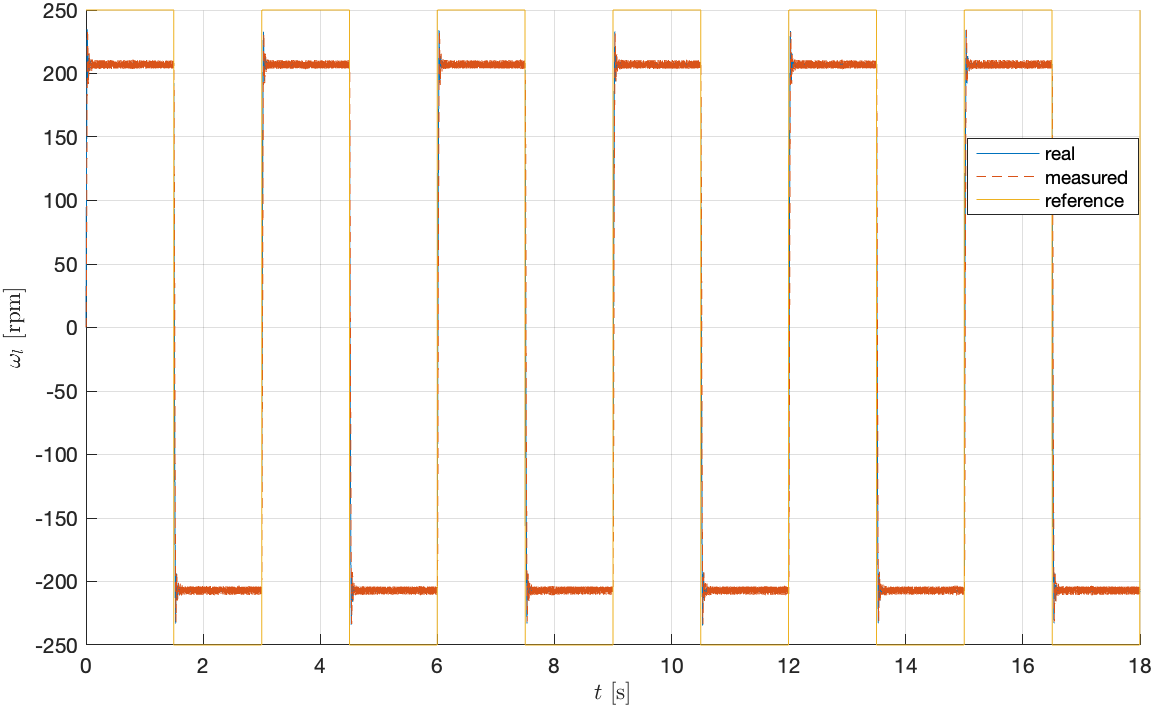
\includegraphics[width=\linewidth]{./Images/Gesu.png}
        \caption{Controllore P}
        \label{Lab5:P}
    \end{subfigure}
    \hfill
    \begin{subfigure}{0.45\linewidth}
        \centering
        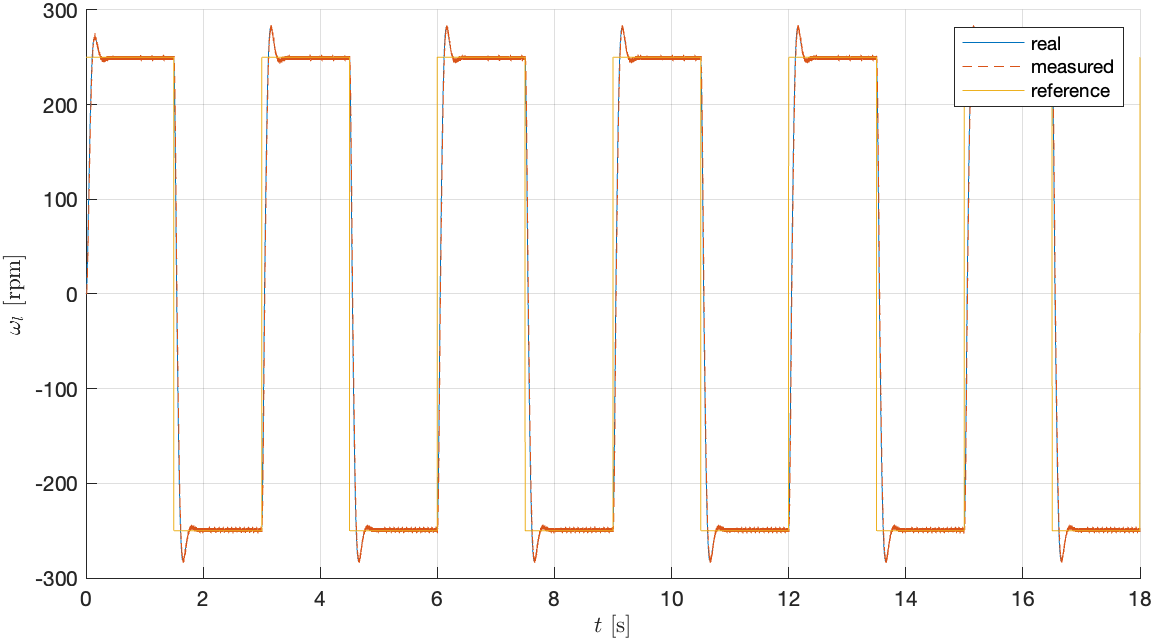
\includegraphics[width=\linewidth]{./Images/Gesu2.png}
        \caption{Controllore PI}
        \label{Lab5:PI}
    \end{subfigure}
    \caption{Simulazione velocità}
\end{figure}

\section{Progettazione controllore PI e verifica sperimentale}
\subsection{Giustificazioni teoriche}
Il controllore da progettare ha delle specifiche da rispettare, in particolare deve garantire l'inseguimento perfetto a regime di un segnale costante e la reiezione dei disturbi costanti dovuti all'attrito. Questo può essere fatto tramite un controllore PI, dato che il polo nell'origine che presenta permette di rendere il sistema retroazionato di tipo 1, dato che il sistema da controllare non ne presenta. Inoltre, garantisce la reiezione di disturbi costanti. 
\subsection{Progettazione a partire dall'approssimazione ai poli dominanti}
Ci sono anche delle specifiche nel dominio del tempo, in particolare il tempo di assestamento al 5\% deve essere $t_{5\%} \le 0.15s$ e la sovraelongazione percentuale deve essere $M_{P} \le 10\%$. Per soddisfare queste caratteristiche, si approssima il sistema in retroazione con uno del secondo ordine, trascurando lo zero che si presenta nella funzione di trasferimento. In questo modo, si possono mettere in relazione le richieste nel dominio del tempo con la pulsazione di attraversamento e il margine di fase. Da queste due, si possono poi ricavare i coefficienti del controllore PI. Cambiando per tentativi i valori scelti, si ottiene $K_{P} = 0.0298$ e $K_{I} = 6.5015$ e, come si può vedere dalla figura \ref{Lab6:Step}, il sistema ha $t_{5\%} = 0.145s$ e $M_{P} = 9.92\%$, soddisfando le richieste originali. A questo punto, si è testato il controllore con il sistema Simulink già sviluppato, in modo da verificare l'effettivo comportamento con il modello completo e non quello semplificato. Si ottiene una sovraelongazione percentuale molto più grande di quella che si trova con il modello semplificato. Probabilmente questo è dovuto al fatto che il sistema presenta delle dinamiche di cui non si è tenuto conto, che abbassano il margine di fase e aumentano la sovraelongazione.
\begin{figure}[H]
    \centering
    \begin{subfigure}{0.4\linewidth}
        \centering
        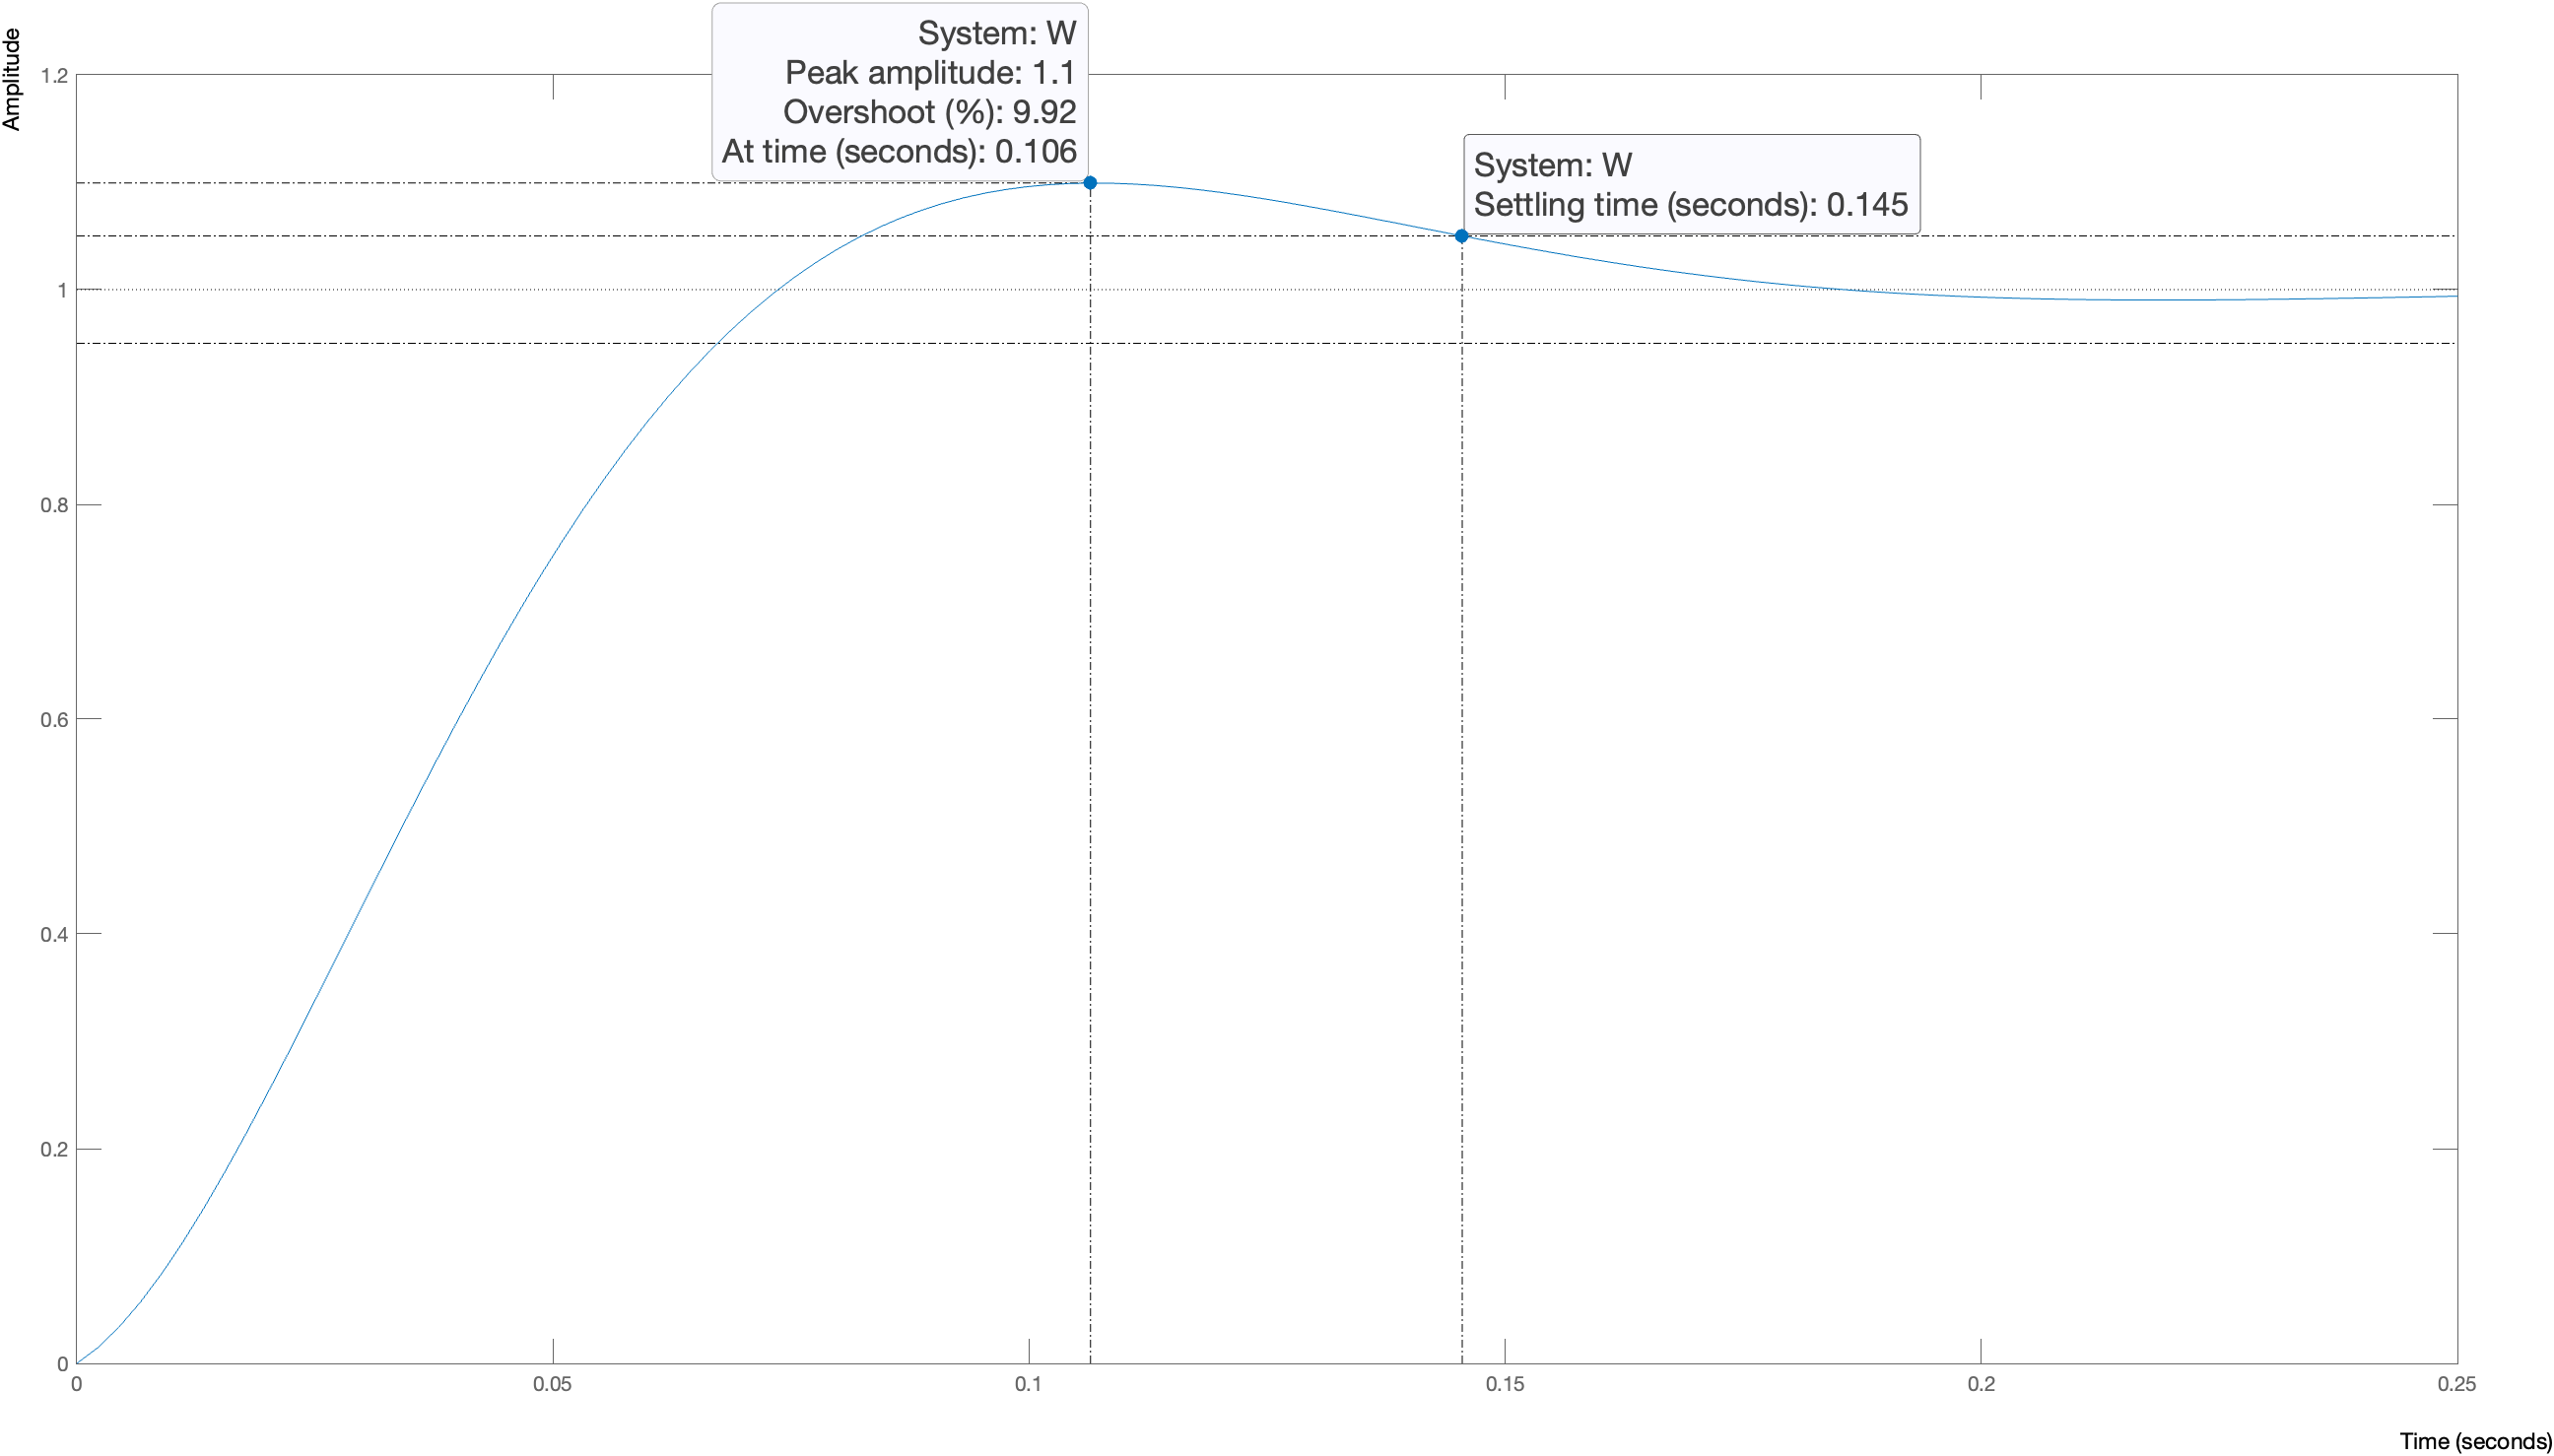
\includegraphics[width=\linewidth]{./Images/Gesu3.png}
        \caption{Risposta al gradino del sistema semplificato in retroazione}
        \label{Lab6:Step}
    \end{subfigure}
    \hfill
    \begin{subfigure}{0.4\linewidth}
        \centering
        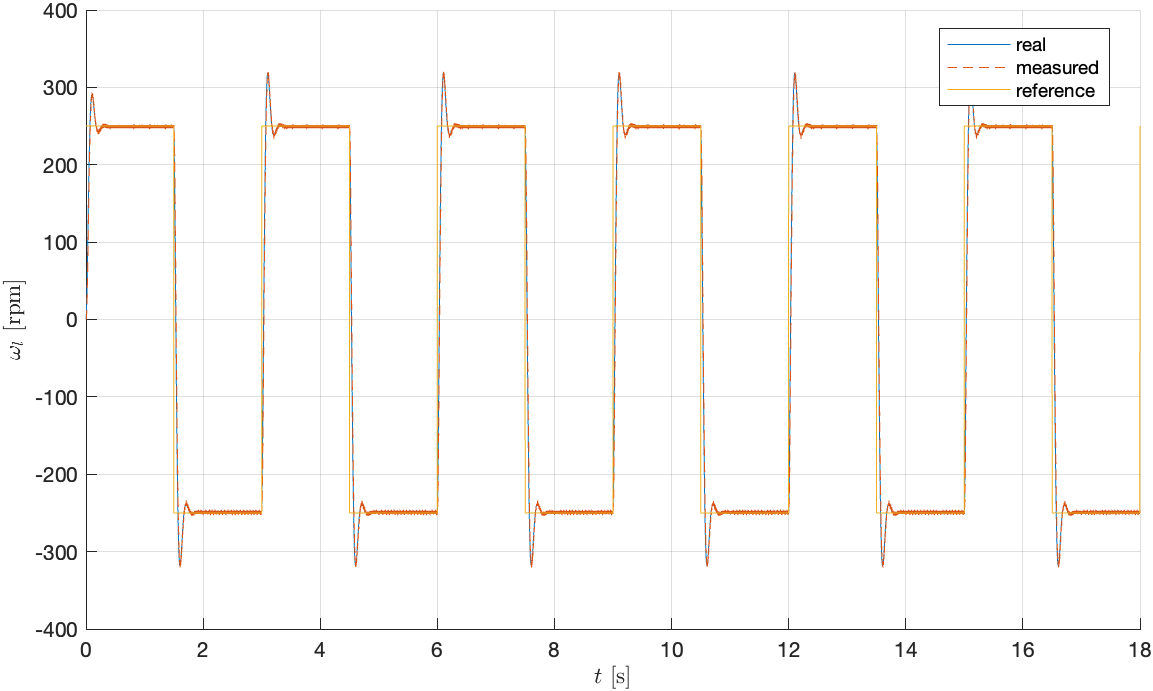
\includegraphics[width=\linewidth]{./Images/Gesu4.png}
        \caption{Risposta a un'onda quadra}
        \label{Lab6:Square}
    \end{subfigure}
    \caption{Simulazione velocità}
\end{figure}

\subsection{Verifica sperimentale in laboratorio}
Si è modificato lo schema Simulink ricorrendo ai blocchi del modulo Simulink Desktop Real-Time, che permette a Matlab di comunicare con il mondo esterno tramite una scheda di acquisizione. Si sono effettuati tre test, con diversi input. Nel primo, si è usata un'onda quadra, con picco $250rpm$ e periodo $3s$. Nel secondo, si è usato un segnale a scalino, con un incremento di $50 rpm$ ogni $5s$ fino a $450rpm$. Il terzo ingresso è un segnale a triangolo, di periodo $2s$ e picco a $450rpm$. Si riportano di seguito i grafici dei risultati della velocità. Dalla figura \ref{Lab1:Square}, si può notare che il risultato sperimentale è molto simile a quello ottenuto per simulazione, confermando la bontà del modello scelto.

\begin{figure}[H]
    \centering
    \begin{subfigure}{0.45\linewidth}
        \centering
        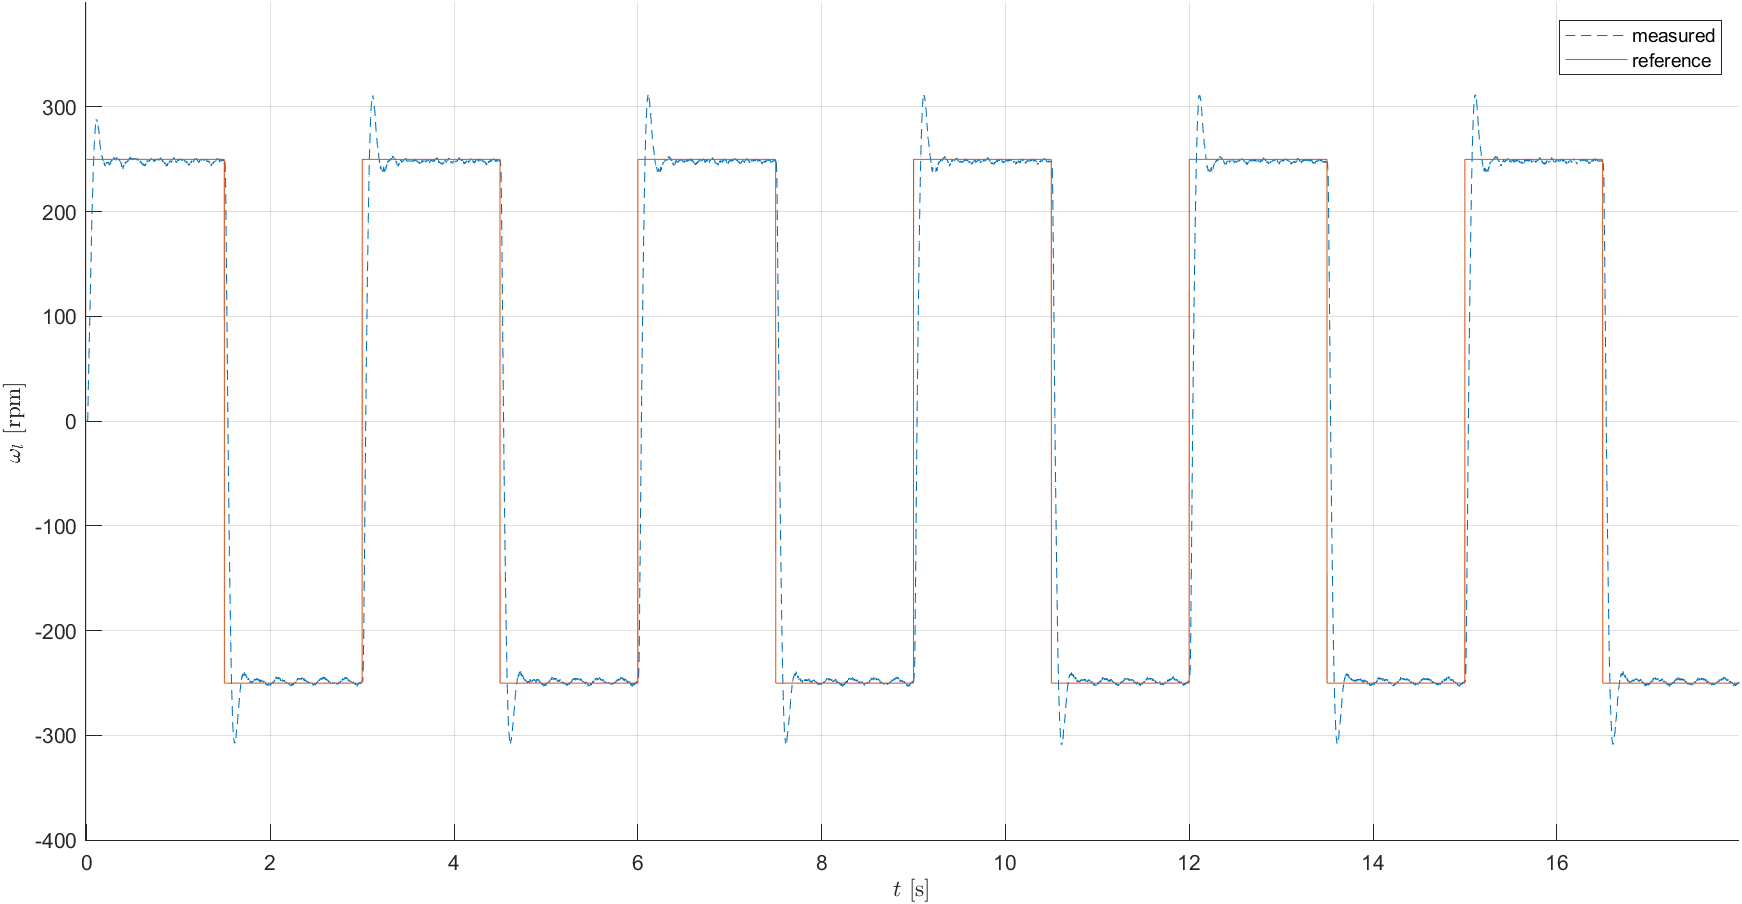
\includegraphics[width=\linewidth]{./Images/MioPadre.png}
        \caption{Ingresso onda quadra}
        \label{Lab1:Square}
    \end{subfigure}
    \hfill
    \begin{subfigure}{0.45\linewidth}
        \centering
        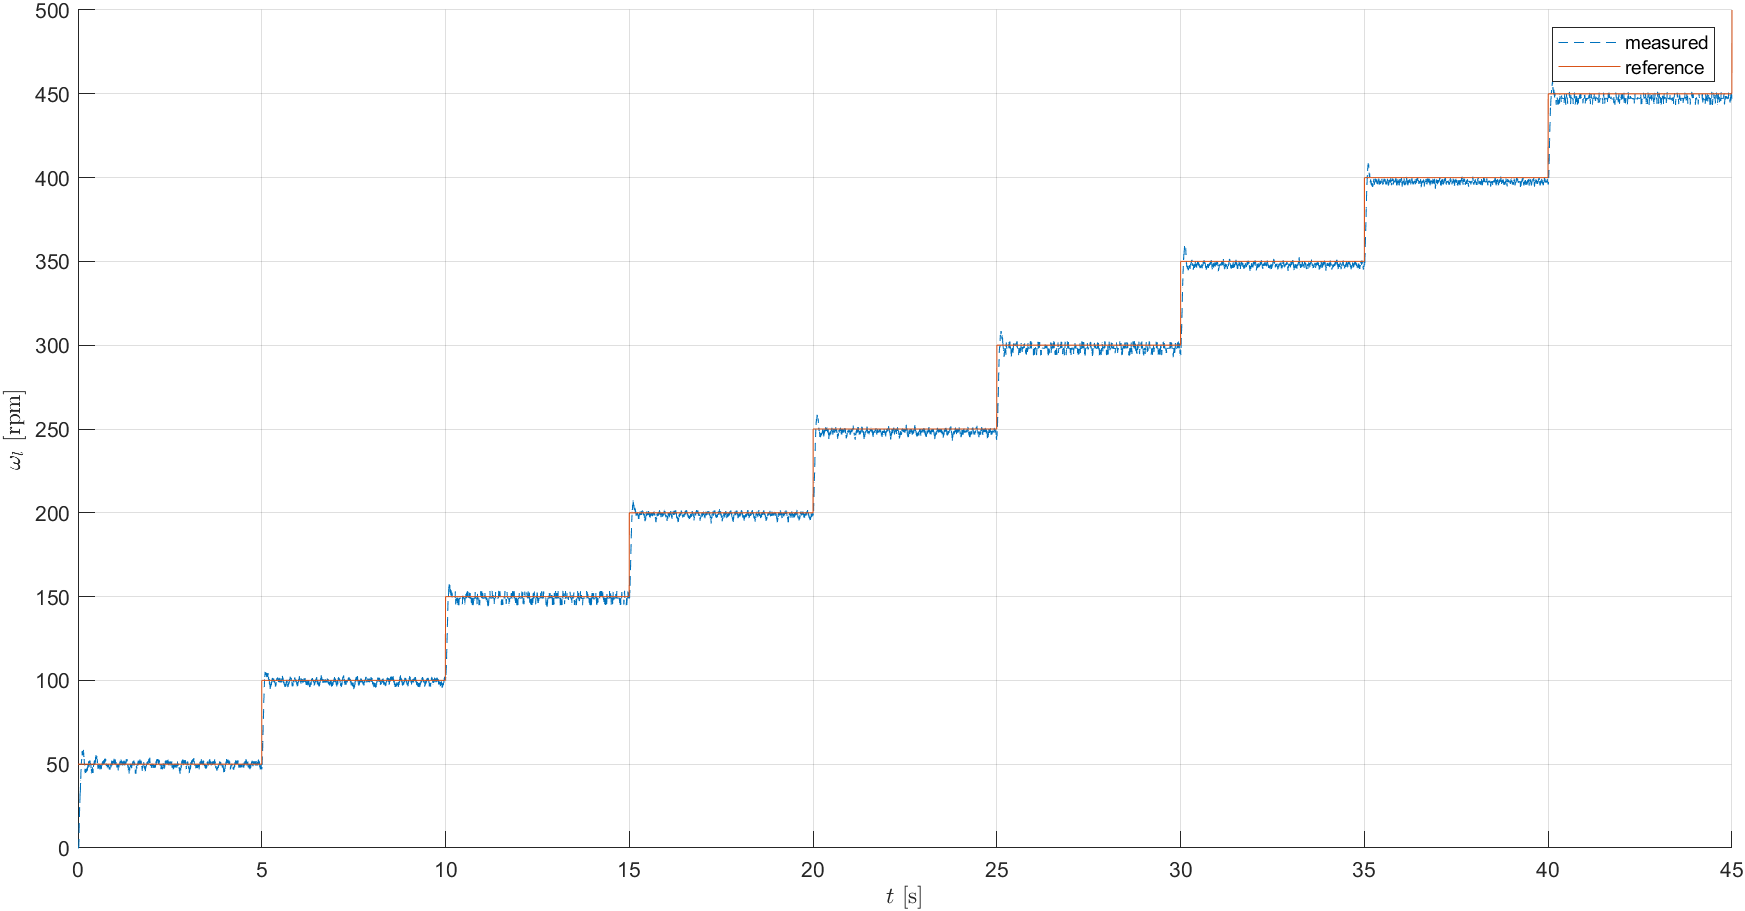
\includegraphics[width=\linewidth]{./Images/MioPadre2.png}
        \caption{Ingresso a scalino positivo}
        \label{Lab1:Stair}
    \end{subfigure}
    \hfill
    \begin{subfigure}{0.45\linewidth}
        \centering
        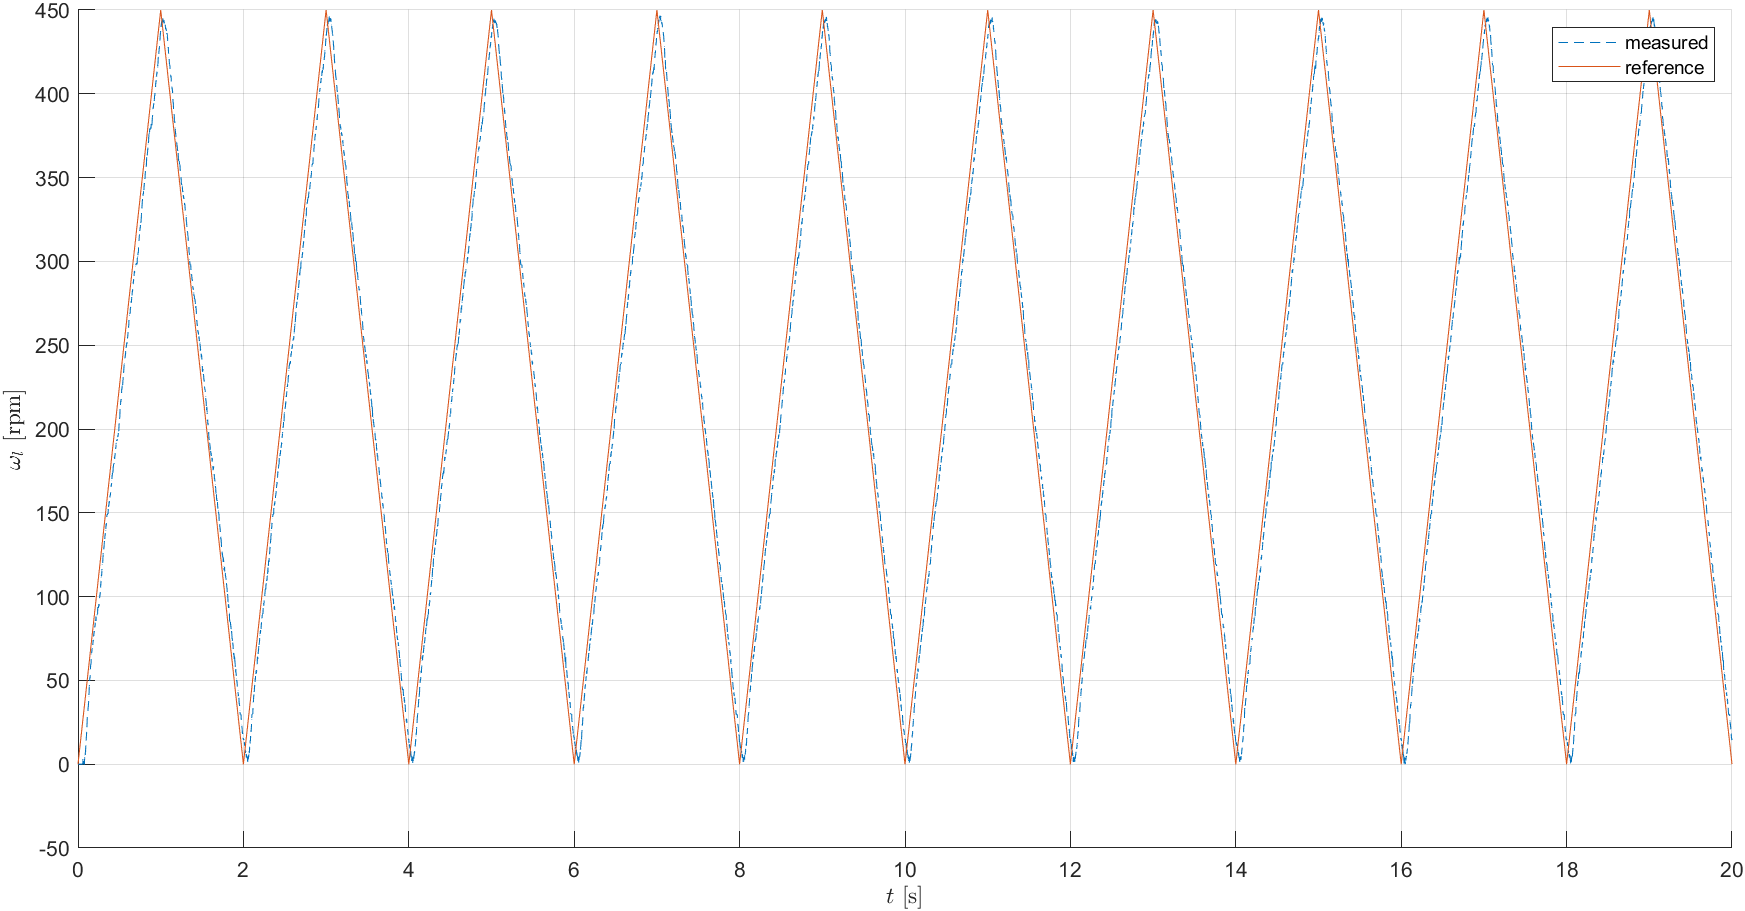
\includegraphics[width=\linewidth]{./Images/MioPadre3.png}
        \caption{Ingresso a triangolo}
        \label{Lab1:Triang}
    \end{subfigure}
    \caption{Simulazione velocità}
\end{figure}

\end{document}
